\documentclass[12pt, titlepage]{article}
\usepackage[utf8x]{inputenc}
\usepackage[english]{babel}
\usepackage[a4paper, top=3cm, bottom=2cm, left=2cm, right=2cm, marginparwidth=1.75cm, headheight=15pt]{geometry}
\usepackage{tabto}
\usepackage{fancyhdr}
\usepackage{titlesec}
\usepackage{float}
\usepackage{graphicx}
\usepackage{caption}
\usepackage[table]{xcolor}
\usepackage{parskip}
\definecolor{light-gray}{gray}{0.15}
\usepackage[colorlinks=true, allcolors=light-gray]{hyperref}

\newcommand{\code}[1]{\texttt{#1}}

\fancyhead[L]{\today}
\fancyhead[C]{SX-Dashboard Documentation}
\fancyhead[R]{MTechHub}
\pagestyle{fancy}

\setcounter{secnumdepth}{4}

\titleformat{\paragraph}
{\normalfont\normalsize\bfseries}{\theparagraph}{1em}{}
\titlespacing*{\paragraph}
{0pt}{3.25ex plus 1ex minus .2ex}{1.5ex plus .2ex}

\title{SX-Dashboard Documentation}
\author{MTechHub}
\date{\today}

\begin{document}

\setlength{\arrayrulewidth}{1.5pt}
\definecolor{table-grey}{gray}{0.90}

\maketitle
\newpage

\pagenumbering{roman}
\tableofcontents
\newpage
\pagenumbering{arabic}

\section{Project Overview}

\subsection{Application Walk-through}

\subsubsection{Adding packages}

Before the application can be run, it's dependencies must be installed. While in the project directory, run:\\
\code{npm install} or \code{yarn}\\
All the packages will be added to the folder /node\_modules. A list of dependencies can be found under ./package.json.

\subsubsection{Running the Application}

While in the project directory, run:\\
\code{npm start} or \code{yarn start}\\
to begin running the application at http://localhost:3000.\\

To build the application, run:\\
\code{npm build} or \code{yarn build}

\subsubsection{Using the Application}

After running the application, visit http://localhost:3000 in your browser. You should be redirected to http://localhost:3000/main/dashboard, and your screen should look similar to figure 1.

\begin{figure}[H]
\centering
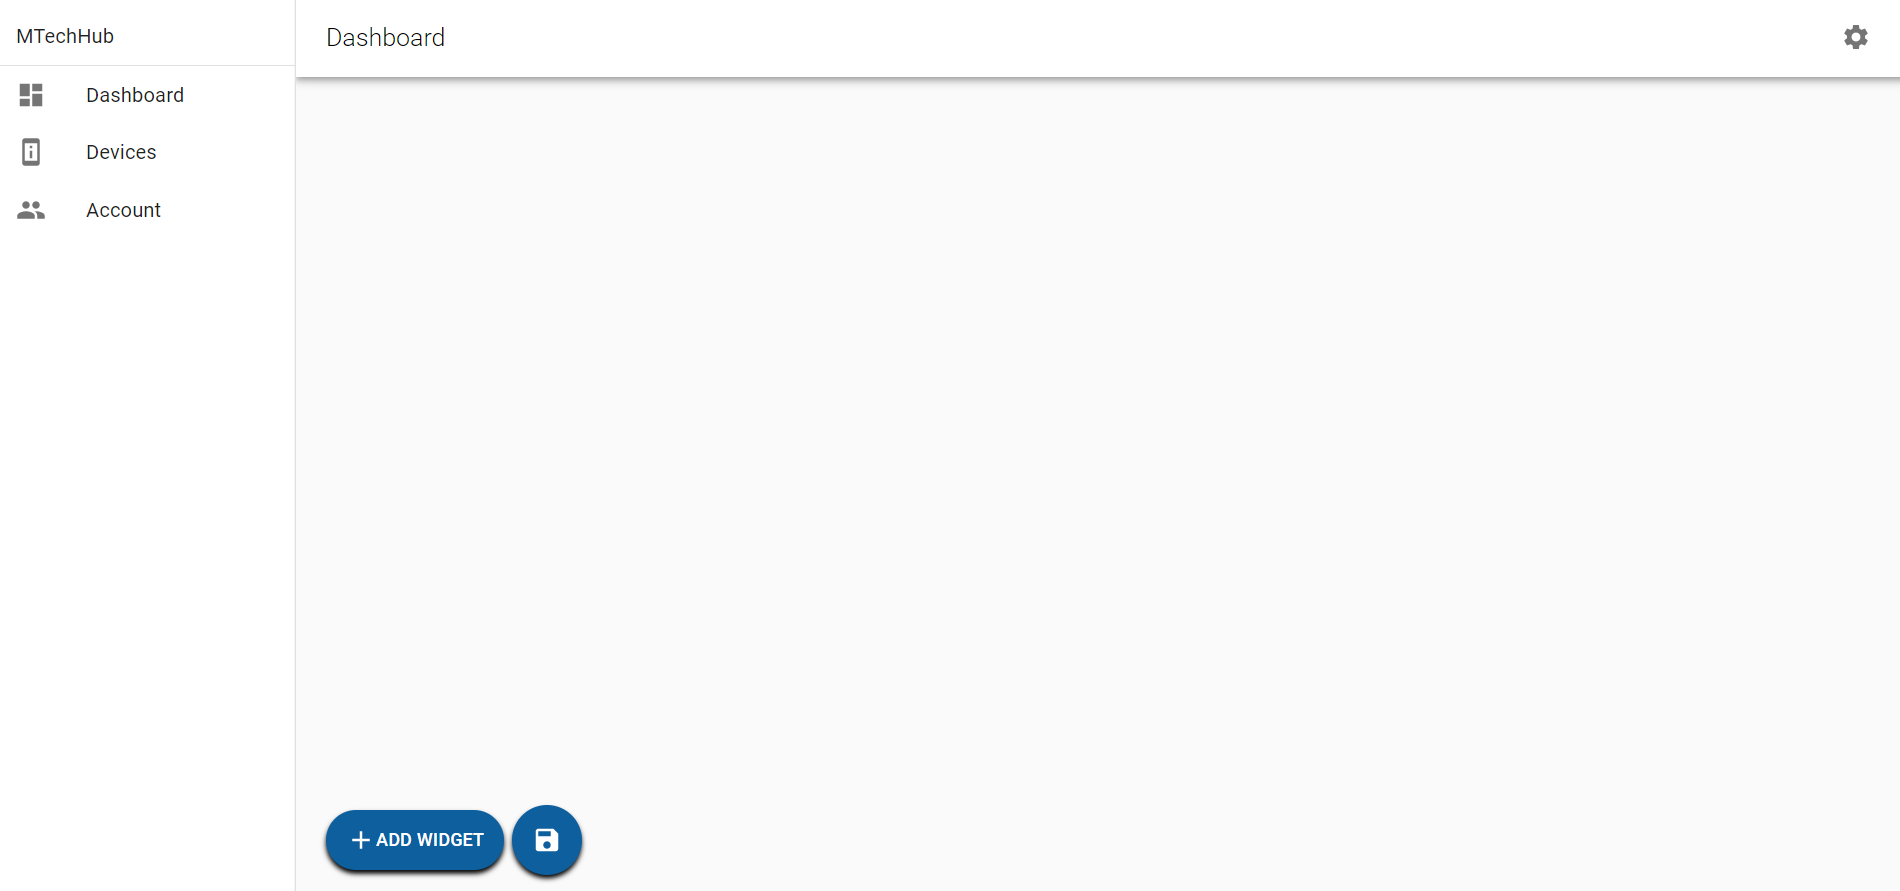
\includegraphics[width=0.9\linewidth]{./assets/Dash.PNG}
\caption{Starting screen}
\label{fig:dash}
\end{figure}



The Devices and Account tabs on the side are placeholders, and should be replaced with required tabs. Selecting Add Widget will bring up a menu with different chart types and a SQL/MQTT slider. The MQTT slider will setup a chart using the MQTT protocol to retrieve live data, whereas the SQL slider will setup a chart using a specified SQL database as the data source. Click the name of the chart you wish to create. A second menu will pop up asking for the relevant data, at the moment this is for show and the logic needs to be implemented. Fill in the required fields and select Create to create a chart.

Note that if creating a chart from SQL, at the moment it will give you a view of the last 10 records in that table, along with the column names so you can select the columns to create the chart from.

A chart should show up on the dashboard. This chart can be manipulated, click and drag to move it, drag the bottom-right corner to resize, and finally press the \textbf{X} in the top-right to delete the chart. Once you are finished with the layout of the dashboard, select the save icon to the right of Add Widget. This will save the layout to SQL, using the server API. At this point, closing the page and re-opening it should load up your last saved dashboard (assuming a successful SQL connection).

There is a cog icon located in the top right corner of the page. Currently this button does nothing, however it can be setup to contain a dropdown allowing theme selection (explained in \_\_\#REF HERE\_\_) as well as any other options that may be required.
\subsection{Code Walk-through}

All of the files mentioned here are found in /src/. Each component will contain a section: 
\begin{verbatim}
    render() {
        return (

        );
    }
\end{verbatim}
\noindent Anything here is what will be rendered whenever this component gets called by another file. The entry point for this project is ./index.js, which contains a router that essentially redirects to ./layout/main.jsx. Main.jsx is the main layout for the project, it just renders the Sidebar component found in ./components/sidebar/sidebar.jsx.

\textbf{The Sidebar Component}

\noindent Sidebar is the menu component found on the left side of the dashboard. When the screen size is md and lower, the menu is hidden and opens via a button placed at the top left of the appbar. The actual items on the sidebar menu are loaded in from ./components/items/. list\_items.jsx is rendered for the persistent sidebar, while mobile\_list\_items.jsx is rendered for the collapsible variant.

\noindent Each of the menu items has an associated path. This path is used in the Router found in the $<$main$>$ section within sidebar.jsx. It essentially loads the content in the main window of the application, and allows that content to change depending on which menu item has been selected.

\textbf{The Dashboard Component}

\noindent The dashboard, located under ./views/dashboard/dashboard.jsx is the default rendered view. componentDidMount() is called as soon as the component is mounted, in here is where we asynchronously make a call to SQL to retrieve the last-saved dashboard layout. In the case that there is no found layout fromm SQL, we attempt to use the last layout stored in localstorage. Else, the dashboard will be a blank slate.

\noindent The createElement function will create a chart for the dashboard using the passed \textit{el} object. 


\subsection{Project Structure}
\subsubsection{doc}

The doc folder contains this pdf and the .tex file used to generate it. Pdflatex is required to regenerate this document locally, however there are compilers online you can use as well if you ever need to make changes. Assets contains the images used in the document.

% ASSETS
\subsubsection{/src/assets}
    \paragraph{css}
    This contains the style sheets used in the project.
    \paragraph{img}
    Images used on the webpage will go here. (MTech Logo should be added and used on the menu)

% COMPONENTS
\subsubsection{/src/components}
    \paragraph{items}

    \paragraph{label}

    \paragraph{popup}

    \paragraph{settings}

    \paragraph{sidebar}

    \paragraph{widgets}

\subsubsection{/src/layout}
    \paragraph{main}

\subsubsection{/src/views}
    \paragraph{account}

    \paragraph{dashboard}

    \paragraph{devices}

\subsection{Libraries}


\section{Things to update}

\end{document}